\documentclass[12pt, letterpaper]{article}
% Reduce the page margins to 3/4 of an inch
\usepackage[margin=0.75in]{geometry}

\usepackage{bookmark}

\usepackage{enumitem}

% References
\usepackage{hyperref}

% Import citations for use with BibTeX
\usepackage{cite}

% Table formatting
\usepackage{tabularx}

% Paragraph-blocks, allowing multi-line cells in tables.
\usepackage{makecell}

% Restrict table of contents to parts through subsubsections
\setcounter{tocdepth}{3}

\usepackage{graphicx}
\hypersetup{
    colorlinks,
    citecolor=black,
    filecolor=black,
    linkcolor=black,
    urlcolor=black
}

\usepackage{fancyhdr}
\pagestyle{fancy}
\fancyhf{}
\rhead{Page \thepage}
\lhead{Software Requirements Specification}
\newcolumntype{R}{>{\raggedleft\arraybackslash}X}%
\fancypagestyle{style1}{
\fancyhf{}
\lhead{Software Requirements Specification}
\rhead{CIOS Digital}
\lfoot{May 16, 2017}
\rfoot{\thepage}

\renewcommand{\headrulewidth}{0.4pt}
\renewcommand{\footrulewidth}{0.4pt}
\newcolumntype{R}{>{\raggedleft\arraybackslash}X}%
}
\fancypagestyle{style2}{
\fancyhf{}
\renewcommand{\headrulewidth}{0pt}
\renewcommand{\footrulewidth}{0pt}
% \rhead{\\}
% \lhead{\\}
\cfoot{\thepage}
%m\renewcommand{\footrulewidth}{0.4pt}
%\newcolumntype{R}{>{\raggedleft\arraybackslash}X}%
}
\pagestyle{style1}

\makeatletter
\renewcommand{\maketitle}{\bgroup\setlength{\parindent}{0pt}
\thispagestyle{empty}
\null
  \begin{flushleft}
  \vspace{15mm}
  \vskip2mm
  \Huge{\textbf{\@title}}
  \vspace{7cm}
\begin{figure}[ht]
  \begin{minipage}[b]{0.45\linewidth}
    
\includegraphics[width=.75\textwidth]{images/cios.png}
  \end{minipage}
  \hspace{0.5cm}
  \begin{minipage}[b][][c]{0.45\linewidth}
    \LARGE{\@author}
  \vspace{0.35cm}
  \end{minipage}
\end{figure}
\\CSCI 492: Spring 2017\\
  \end{flushleft}\egroup
}
\makeatother

\title{Software Requirements Specification\\for\\Flight Plan Editor}
\date{}
\author{
Cedrick Cooke\\
Ian Littke\\
Owen Roth-Lerner\\
Sander Scherman Garzon\\
}

\begin{document}
\pagenumbering{roman}
\maketitle

\newpage
\pagestyle{style2}
\setcounter{page}{1}
\section*{Revision History}
\begin{tabularx}{\textwidth}{l r X l}
\textbf{Name} & \textbf{Date} & \textbf{Reason for Change} & \textbf{Version} \\
\hline
\hline
Ian Littke & 2017-02-21 & Initial document blocking & 0.1 \\
\makecell[cl]{Cedrick Cooke,\\ Owen Roth-Lerner,\\ Sander Scherman Garzon} & 2017-02-23 & Expanded sections 3 and 4 & 0.2 \\
Ian Litke & 2017-05-16 & Reformat Document & 0.3 \\
          % &            &                   &     \\
          % &            &                   &     \\
          % &            &                   &     \\
          % &            &                   &     \\
          % &            &                   &     \\
          % &            &                   &     \\
          % &            &                   &     \\
          % &            &                   &     \\
          % &            &                   &     \\
          \hline
\end{tabularx}

\newpage

\tableofcontents
\newpage
\pagenumbering{arabic}
\pagestyle{style1}
\setcounter{page}{1}

\section{Introduction}
  \subsection{Purpose}
    This SRS describes the software functional and nonfunctional requirements
    for release 1.0 of the Flight Plan Editor.
    This document is intended to be used by the members of the project team that will implement
    and verify the correct functioning of the system.
    Unless otherwise noted, all requirements specified here are high priority
    and committed for release 1.0.
  \subsection{Document Conventions}
  This document features some terminology which readers may be unfamiliar with.
  See \hyperref[sec:glossary]{Appendix \ref{sec:glossary} (Glossary)} for a list of these terms and their definitions.
  The format of this SRS is simple. Bold face and indentation is used on general topics and or specific points of interest.
  Font style is Computer Modern and the document is typset using \LaTeX;
  \subsection{Intended Audience and Reading Suggestions}
  This document is intended for all individuals participating in the initial release of Flight Plan Editor.
  Including, but not limited to, all project team members; Aran Clauson, team mentor; and Martin Kjelstad, CAP contact point.

  \subsection{Project Scope}
  The Flight Planning Editor will allow flight planners in the Civilian Air Patrol (CAP)
  to create their flight plans in a graphical interface and store them on a Secure Digital (SD) card.
  A detailed project description is available in the \hyperref[sec:ref]{\textit{Flight Plan Editor Vision and Scope Document}}.
  The section in that document titled "Scope of Initial and Subsequent Releases" lists the features that are
  scheduled for full or partial implementation in this release.

  \subsection{Definitions, acronyms, and abbreviations} \label{sec:glossary}
\begin{description}[style=nextline, leftmargin=10mm, topsep=0mm,noitemsep]
      \item[CAP] \hfill \ Civilian Air Patrol
      \item[FAA] \hfill \ Federal Aviation Administration
      \item[Garmin G1000] \hfill \ Integratead flight instrumentation system used in planes
      \item[GeoTIFF] \hfill \ Metadata standard which allows georeferenceing information to be embedded within a TIFF file
      \item[GPS] \hfill \ Global Positioning System
      \item[Sectional] \hfill \ Sectioned chart covering a section of an area, usually by state
      \item[SRS] \hfill \ Software Requirements Specification
      \item[SD Card] \hfill \ Secure Digital Card
      \item[TIFF] \hfill \ Tagged Image File Format
      \item[VFR] \hfill \ Visual Flight Rules
      \item[XML] \hfill \ eXtensible Markup Language
  \end{description}

  \subsection{References}\label{sec:ref}
  \begin{tabularx}{\textwidth}{l|X}
    \hline
    Vision and Scope & \url{https://github.com/cedrickcooke/flight-planning/tree/master/vision-scope}\\
    FAA VFR Raster Charts & \url{https://www.faa.gov/air_traffic/flight_info/aeronav/digital_products/vfr/} \\
    \hline
  \end{tabularx}

  \newpage
\section{Overall Description}
  This section gives an overview of the proposed functionality of the product.
  It describes the informal requirements and is used to establish a context for the technical
  requirements specification in the next section.
  \subsection{Product Perspective}
    This flight planning editor addresses a CAP emergency flight planning need.
    Specifically, this new software whill allow a user to input latitude and longitude coordinates
    and view them on a map to develop flight plans.
    These flight plans can then be used in the Garmin G1000 navigation system.
  \subsection{Product Features}
    The most important feature of this product is the ability to read, edit, and write XML containing flight plans.
    This is accomplished through a user interface in which allow the user will enter coordinates which are then
    displayed on a map for reviewing and modification.
    Once the flight plan is finished, the user can save their plan to the SD card to be used in the G1000.
  \subsection{User Classes and Characteristics}
    There is only one type of user that will interact with the system:
    users that have the authority to create flight-plans.
    In the case of the Bellingham CAP, this is limited to two people.
    The user is expected to have knowledge of flying area and can read charts.
    The user shall also be expected to have lattitude-longitude coordinates of
    waypoints of interest to include in the flight plan.
  \subsection{Operating Environment}
      The system will be able to run on Microsoft Windows products, starting with Windows 7.
      The system only focuses on Windows due to the availability of Windows machines utilized by the CAP.
  \subsection{Design and Implementation Constraints}
      The system's design and code shall be written in C\#.\\
      User interface shall be written in XAML for Windows Presentation Foundation.\\
      All flight plans shall be recorded in XML.\\
    \end{tabularx}
  \subsection{User Documentation}
      The system shall provide hierarchiacal and cross-linked help system in HTML that
              describes and illustrates all system functions.\\
      The system shall also offer tooltips to assist in user functions \\
  \subsection{Assumptions and Dependencies}
      \subsubsection{Assumptions}
       Flight operators can map around restricted areas/altitude.
       The system will not alert the user if a flight path passes through restricted airspace or through a mountain.
       It it remaines up to the user to be able to through these issues.

       It is a dependency that the SD card used to save the flight plans on are of the same make/model that
       is able to be read by the G1000 system.

    \newpage

    \subsection{Input Destination Coordinates}

      \subsubsection{Description and Priority}
  		In the top left corner of the application, there are two input windows for
  		lattitude/longitude coordinate input. Once the user enters the data,
  		points on the sectional map will appear as well as a text list for each
  		coordinate.
      \subsubsection{Stimulus/Response Sequences}
        \begin{description}
          \item[Stimulus] User will click on the lattitude text box to input the
  			lattitude, and complete the same for longitude.
        \begin{description}[0.2cm]
  		\item[Response] Upon completion, the user will hit the enter key on their
  			keyboard, and the map shall display the point respective
  			to the lattitude/longitude input.
      \end{description}
  		\item[Stimulus] User can then request to edit an existing waypoint.
  		\item[Response] The coordinate is displayed, and user will have the option to
  			either save or discard the changes.
        \end{description}
      \subsubsection{Functional Requirements}
      \begin{tabularx}{\textwidth}{|l|X|} \hline
        FR-4: & There will be a text input box for both lattitude and longtitude coordinate input\\ \hline
        FR-5: & Upon entering coordinates, a waypoint will be drawn on the sectional map to represent its location\\ \hline
        FR-6: & Selecting an already created waypoint allows the user to modify the coordinates, or discard the waypoint\\ \hline
        \end{tabularx}

\section{System Features}
  \subsection{Display Sectional Map}
    \subsubsection{Description and Priority}
      The application will display the sectional map as the main interface.
      The map will respond to input from lattitude/longitude coordinate input as well
      as having the ability to pan around the map.
    \subsubsection{Requirements}
      \begin{description}
        \item[r1.1] A user can request to create a new waypoint via a textbox.
		\item[r1.2]	The sectional map will create a new point on the map to
			reflect the changes made.
		\item[Stimulus] A user can also click on the map and drag their mouse
			across the screen.
    \item[Response] The program will adjust the view of the map vertically and horizontally,
			in the opposite direction of the mouse pointers movement.
		\item[Stimulus] A user may also scroll with the mousewheel.
		\item[Response] The map will either zoom in or zoom out depending on the mouse scroll.
      \end{description}
    \subsubsection{Functional Requirements}
    \begin{tabularx}{\textwidth}{|l|X|} \hline
      FR-1: & Upon starting the program, the sectional map will be displayed\\ \hline
      FR-2: & This map will have the ability to maneuver and pan based upon user mouse movement\\ \hline
      FR-3: & Map will also respond to changes in waypoints, or selecting different flight plans\\ \hline
      \end{tabularx}



    \subsection{Distinguish Waypoint Coordinates}
      \subsubsection{Description and Priority}
		As a user inputs more lattitude/longitude coordinates, the program will
	    draw a new waypoint onto the sectional map for viewing as well
		as having a small subtext containing the lattitude/longitude coordinates
		for viewing to distinguish each waypoint. Priority = medium.
      \subsubsection{Stimulus/Response Sequences}
        \begin{description}
          \item[Stimulus] A user can request to view the listed waypoints on the map.
		  \item[Response] The program will display the lattitude/longitude data
			for that given point on the sectional map, as well as highlight the
			list of waypoints that were already added to that particular flight
			plan.
        \end{description}
      \subsubsection{Functional Requirements}
      \begin{tabularx}{\textwidth}{|l|X|} \hline
        FR-7: & Each waypoint drawn on the map shall display the lattitude and longitude coordinates\\ \hline
        FR-8: & Each waypoint will also be displayed as a list between other points for connections\\ \hline
        \end{tabularx}


      \subsection{Draw Flight Path on Section Map Between Coordinates}
        \subsubsection{Description and Priority}
        		The user should have the ability to not only add or delete points, but change in which
        		order he connects one point to another. This allows the user to actually route between
        		points rather than have to manually navigate between them. (Priority = High)
        \subsubsection{Stimulus/Response Sequences}
            Upon selection/editing a flight plan, the program will pull up a list of previous flight
            points and the path between them on a map. These points will be pathed in the order the
            appear on the list, and changing the order will change what point each point connects to.
            The user will be able to see this editing of order (and thereby flight path) automatically
            on the map.
        \subsubsection{Functional Requirements}
          \begin{tabularx}{\textwidth}{|l|X|} \hline
            FR-9: & The point list shall have ability to edit ordering of lat/long coordinates\\ \hline
            FR-10: & If adding new lat/long coordinates, the previous coord will connect to new one.\\ \hline
            FR-11: & If coordinate is last on list, the path will end there.\\ \hline
      	    FR-12: & The map shall update to show new path as the list is edited/extended.\\ \hline
          \end{tabularx}
        \subsection{Open and Save Flight Plan in XML to SD Card}
          \subsubsection{Description and Priority}
            The Garmin G1000 uses SD cards to store flight plans, and does so in the XML format.
            For this program to be of any use, it \emph{must} support reading and writing these files.
            Priority = High
          \subsubsection{Stimulus/Response Sequences}
            \paragraph{Opening a file:}
            \begin{description}
              \item[Step 1] User initiates an open action.
              \item[Step 1.1] If the user has an unsaved, open flight plan, prompt the user if they want to save it.
                If the user chooses to save the plan, complete the `saving a file' section before continuing.
              \item[Step 2] User is prompted to select a file to open.
              \item[Step 3] The file is deserialized and displayed.
              \item[Step 3.1] If the file is invalid, corrupt, or otherwise fails to open, display a warning to the user.
            \end{description}
            \paragraph{Saving a file:}
            \begin{description}
              \item[Step 1] User initiates a save action or a save-as action.
              \item[Step 2] If the user selected a save-as action, or if the current plan is not already associated with a file,
                the user selects the file location and file name they would like to use.
              \item[Step 3] The current flight plan is serialized to XML, and written to the file.
              \item[Step 4] After writing the file completes, a message is displayed to alert the user.
            \end{description}
          \subsubsection{Functional Requirements}
            \begin{description}
              \item[FlightPlan.XML.Open] The program shall let a user open files. \\
              \item[FlightPlan.XML.Open.Select] The program shall prompt the user to select a file to open. \\ \
              \item[FlightPlan.XML.Open.Failure] After a plan is selected to open, if it fails, the user shall be alerted to the failure. \\
              \item[FlightPlan.XML.Open.Success] After a plan is selected to open, if it succeeds, the user interface should automatically update to reflect the plan. \\
              \item[FlightPlan.XML.Save] The program shall let a user save files. \\ \
              \item[FlightPlan.XML.Save.Select] If the program cannot detect where the file was opened from,
                         or if the save-as option was used to initiate the save, the program shall prompt a user for a location to save the file. \\
              \item[ FlightPlan.XML.Save.Failure] If an attempt to save a file fails, the user shall be alerted to the failure. \\
              \item[FlightPlan.XML.Save.Success] If an attempt to save a file succeeds, the program shall display a message indicating the success. \\
            \end{description}
          \newpage
\section{External Interface Requirements}
  This section provides a description of all inputs into and outputs from the system.
  It also gives a description of the software and communication interfaces and provides a basic prototype of the user interface.
\subsection{User Interfaces}
  The user interface is divided into two main sections: the map view on the right and waypoint editing on the left.
  The user may load up previously saved flight plans or create a new plan as well as modify the current selected plan.
  \begin{figure}[!ht]
    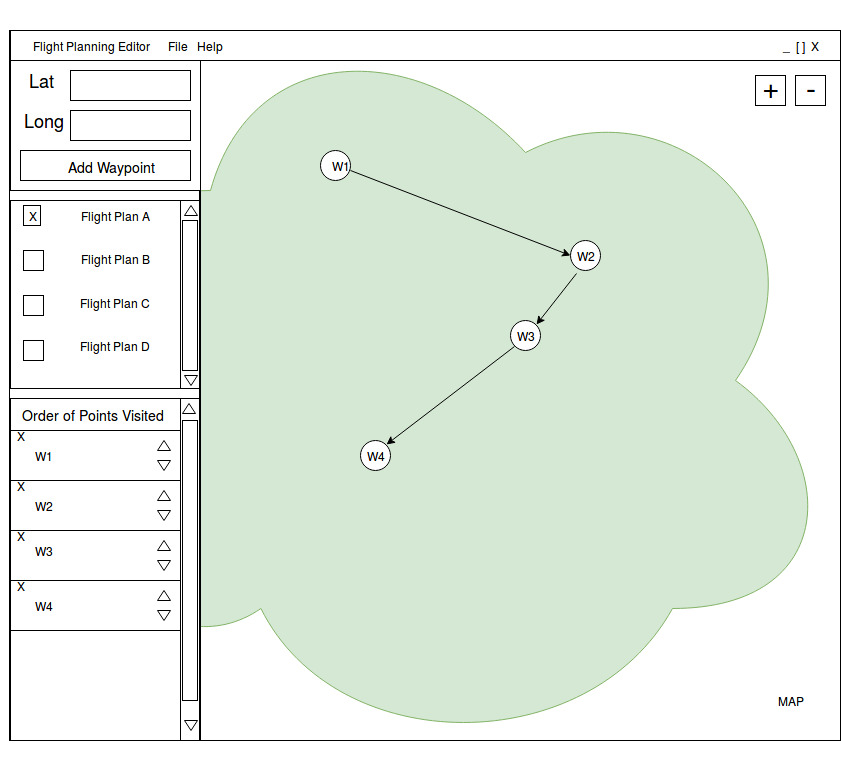
\includegraphics[scale=0.5]{images/FlightPlanning_Interface.jpg}
  \end{figure}

  \subsection{Hardware Interfaces}
    There are no direct hardware interfaces, however the flight plans that are saved must be able to written to SD card.

    \subsection{Software Interfaces}
     No software interface requirements have been identified at this time.
  \subsection{Communications Interfaces}
  No communications interfaces exist.

  \subsection{Performance Requirements}
  The user interface should be able to render the maps within 1 minute of request from the user.

  \subsection{Safety Requirments}
  No safety requirements have been identified.
  \subsection{Security Requirements}
  No security requirements have been identified.
  \subsection{Software Quality Attributes}
	No additional software quality attributes at this time.

% \newpage
%   \appendix
%
% \section{Analysis Models}
%
% \section{Issues List}
%
% \bibliography{citations}{}
% \bibliographystyle{plain}
\end{document}
